\documentclass[12pt]{article}
\setlength\parindent{0pt}
\usepackage{fullpage}
\usepackage{amsmath}
\usepackage{hyperref}
\usepackage{graphicx}
\setlength{\parskip}{4mm}
\def\LL{\left\langle}   % left angle bracket
\def\RR{\right\rangle}  % right angle bracket
\def\LP{\left(}         % left parenthesis
\def\RP{\right)}        % right parenthesis
\def\LB{\left\{}        % left curly bracket
\def\RB{\right\}}       % right curly bracket
\def\PAR#1#2{ {{\partial #1}\over{\partial #2}} }
\def\PARTWO#1#2{ {{\partial^2 #1}\over{\partial #2}^2} }
\def\PARTWOMIX#1#2#3{ {{\partial^2 #1}\over{\partial #2 \partial #3}} }
\newcommand{\BE}{\begin{displaymath}}
\newcommand{\EE}{\end{displaymath}}
\newcommand{\BNE}{\begin{equation}}
\newcommand{\ENE}{\end{equation}}
\newcommand{\BEA}{\begin{eqnarray}}
\newcommand{\EEA}{\nonumber\end{eqnarray}}
\newcommand{\EL}{\nonumber\\}
\newcommand{\la}[1]{\label{#1}}
\newcommand{\ie}{{\em i.e.\ }}
\newcommand{\eg}{{\em e.\,g.\ }}
\newcommand{\cf}{cf.\ }
\newcommand{\etc}{etc.\ }
\newcommand{\Tr}{{\rm tr}}
\newcommand{\etal}{{\it et al.}}
\newcommand{\OL}[1]{\overline{#1}\ } % overline
\newcommand{\OLL}[1]{\overline{\overline{#1}}\ } % double overline
\newcommand{\OON}{\frac{1}{N}} % "one over N"
\newcommand{\OOX}[1]{\frac{1}{#1}} % "one over X"

\pagenumbering{gobble}

\begin{document}
\Large
\centerline{\sc{Homework 4}}
\normalsize
\centerline{\sc{Due in recitation on Friday, March 4}}

{\sc Note:} For all problems, in order to receive credit, you must draw force diagrams for all relevant objects. These diagrams must be at least two inches tall to receive full credit.
This is for your benefit, not mine; carefully drawing clear diagrams will help you with these problems more than anything else.

\vspace{1em}

\begin{enumerate}


  \begin{minipage}{0.7\textwidth}
\item  An object of mass $M$ sits on a frictionless table; it is connected by
   a light string to a hanging mass $m$. (See figure.)
\begin{enumerate}
\item Find both the tension in the string and the acceleration of the masses in terms of $M$, $m$, and $g$.
\item What is the tension in the limit where $M \gg m$ (that is, the mass on the table is very heavy)? Is this what you expect it to be?
\item What is the acceleration in the limit where $m \gg M$ (that is, the hanging mass is very heavy)? Is this what you expect it to be? Think about two cases: (i) $M$ is a bowling ball and $m$ is a feather, and (ii) $M$ is a feather and $m$ is a bowling ball.
\end{enumerate}
  \end{minipage}
  \begin{minipage}{0.3\textwidth}
\centerline{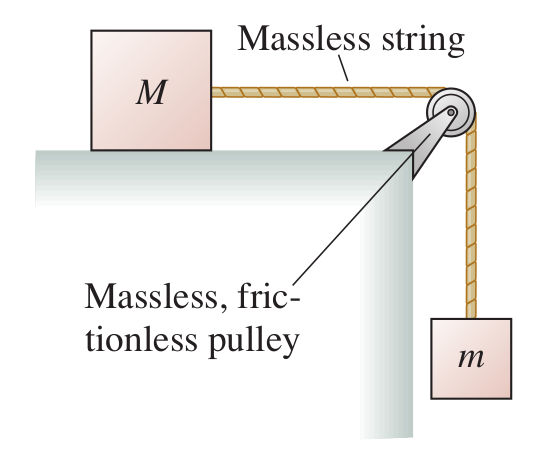
\includegraphics[width=0.9\textwidth]{problem736.png}}
  \end{minipage}

\bigskip

  \begin{minipage}{0.7\textwidth}
\item Two masses are connected by a light string and draped over a light, frictionless pulley. One has mass $m$, which you will find; the other has mass $M=100$ kg. (See figure.)
   
\begin{enumerate}
\item Find an expression for the acceleration of the mass $M$ in terms of $M$, $m$,
and $g$.
\item If it takes a time $\tau=7$ s to hit the ground after it is released, what is
the value of $m$? 
\end{enumerate}
  \end{minipage}
  \begin{minipage}{0.3\textwidth}
\centerline{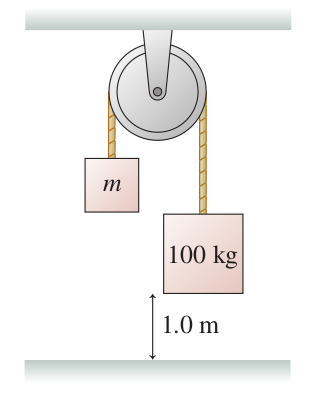
\includegraphics[width=0.9\textwidth]{problem738.png}}
  \end{minipage}

\newpage

\bigskip

  \begin{minipage}{0.6\textwidth}
\item A rope-and-pulley system is set up as shown.
   
  \end{minipage}
  \begin{minipage}{0.4\textwidth}
\centerline{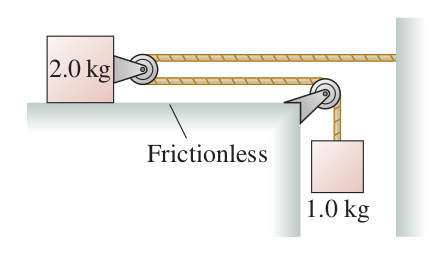
\includegraphics[width=0.9\textwidth]{problem755.png}}
  \end{minipage}

\begin{enumerate} 
	
	\item How does the acceleration of the two blocks relate? ({\it Hint: If the hanging mass moves downward by one meter, how far does the block on the table
move?})

    \item  What is the acceleration of the 
    2 kg block sitting on the table? 
    \end{enumerate}

\bigskip


  \item{A block of mass $m_1=5$ kg rests on a table. Two ropes connect that block to two masses: one hangs off the left side of the table, and the other hangs off the
right side.  The coefficient of static friction $\mu_s$ between the block and the table is 0.2.\\
    
    If one of the hanging masses has mass $m_2=3$ kg, for what range of values of the other block's mass $m_3$ will the system not move?\\
  
  {\sc Hint}: What happens if $m_3$ is very small? What happens if it is very big? Does this affect your force diagram in any way? How do you know what direction
static friction will point? Does this depend on the sizes of the masses? You will need to think carefully about this, possibly making two diagrams depending on the direction of friction.

}

\bigskip

\item{Two blocks connected by a cable slide down an incline angled at $30^\circ$ above the horizontal, connected by a cable. The top block has a mass of $m_1=1$ kg, and the bottom one has a mass of $m_2=2$ kg. The coefficients of kinetic friction are 
  $\mu_{k_1}=0.2$ (top block) and $\mu_{k_2}=0.1$ (bottom block). What is the tension in the cable that connects them?}


\bigskip

\item{A hiker with a mass of 75 kg wants to drag a 180 kg sled over snow at a constant rate. She does this by tying a rope to the sled (at ground level) and running it over her shoulder. The rope running between her and the sled makes a 45 degree angle with the horizontal.

  If the coefficient of friction between the sled and the snow is 0.1, what must the coefficient of friction between her boots and the ground be for her to move the sled?}

\begin{itemize}
\item {\sc Hint 1:} Think carefully about which way the force of friction points on the hiker. 
\item {\sc Hint 2:} This problem will quickly get out of hand if you are not organized. Start by drawing force diagrams for both objects. Then write down $\sum F = ma$ in each direction for each object. This will generate a system of four equations with four unknowns which you will need to solve {\bf by substitution}.
\item {\sc Hint 3:} Solving this system is easiest to do ``back to front'', starting with the $y-$equation for the sled, then the $x-$equation for the sled, then the $y-$equation for the hiker, and finally the $x-$equation for the hiker.
\end{itemize}


%\item See Problem 2 on the first practice exam, at \url{https://walterfreeman.github.io/phy211/practice-exam-1-all.pdf}.
%
%\begin{itemize}
%\item In this problem, is the car experiencing static or kinetic friction while on the snow? Is it experiencing static or 
%kinetic friction on the ice?
%\item If the hill has a slope of $15^\circ$, determine the coefficient of friction on the snow, and on the ice. (I 
%wound up making up nice and simple numbers for you to do this problem; it turns out this car has some very nice snow tires!)
%\end{itemize}

%\item I drive a small sedan (a 2009 Toyota Yaris) that is front wheel drive. This means that the engine is linked only to the front wheels, so only the static friction coming from the front wheels can provide traction to help me move forward.
%
%However, it has brakes on all four wheels, so static friction from both the front and the back wheels can provide traction to help me stop.
%
%Since the engine is the heaviest part of the car, the front wheels bear most of the car's weight. For this problem, assume
%that the front wheels supply 2/3 of the normal force and the rear wheels supply the other 1/3.
%
%In the summer of 2017, I was driving this car on some steep and dusty mountain roads ($\mu_s = 0.7$) in the mountains in Colorado. When I was climbing up the mountains, I was confident that I could make it safely back down any slope that I could 
%climb up. However, I knew the reverse wasn't true, and was very reluctant to drive {\it down} a steep slope since
%I didn't know if I could make it back up.
%
%\begin{itemize}
%\item What is the steepest slope that my car can drive up (at a constant velocity)?
%\item What is the steepest slope that my car can travel down safely (without sliding down the slope)?
%\item Will four wheel drive help you avoid a car accident on icy roads in Syracuse? Will it help you avoid getting your 
%car stuck?
%\end{itemize}



    \end{enumerate}
\end{document}
